\chapter{Cortical Bone}

\section{Introduction following biological literature}
\textit{Extracted from P\&G Paper, 2009} Cortical Bone is a highly organized hard tissue representing approximately 80\% of the skeletal mass in an human adult. The standard description associated to a mechanical point of view is defining it as a two-phase composite material: a soft phase mainly of pores, containing fluid and soft tissues as cells, blood vessels, and a complex hard matrix phase with nerves distributed inside. Such a matrix consist mainly of hidroxyapatite and collagen. Porosity is distributed over various lenght scales, nevertheless only the two largest pores types: resorption cavities (with size of approx. $50-200 [\mu m]$ and Haversian canal (size of approx. $50 [ \mu m ]$ contribute to the so-called mesoscale stucture, hence the mesoscale porosity which is characteristic of the higher level of organization in bone. 

\textit{Extracted from Panrll, Vu, Grimal, Naili, 2011} \\
From a mechanical point of view, bone is a relatively hard and lightweight composite material defined by and hierarchy of microstructures. Scaling down to manometers we observe important functional structures for the cortical tissue such as: Haversian systems and osteons, lamellae, collagen fibres, collagen fibrils and elementary constituents (such as mineral, collagen, water, etc.).\\
From a compositional point of view, the constituents are given by: an organic phase, mainly made of collagen (of type-I); a mineral phase, composed primary of hydroxyapatite crystals; and a fluid phase (water and organic fluids), partially filling the micro- and macro-composites.

\section{Introduction from multiscale literature}
\textit{Ideas from: Multiscale modelling of weakly. Caiazzo, Mura, 2014}
Computational modelling of biological tissues (in particular of bone) is a complex multiscale problem, since there are multiple physical phenomena interacting at various scales. Since in a bast majority of clinical applications the material are viewed as continuum, it's important to contribute in a mathematical model and numerical procedure to characterize non-trivial properties arising from the microscopic physical and geometrical structures affecting the overall behavior, in terms of effective compresibility (or viscosity) or elasticity. 

Nowadays, noninvasive resonance technique corresponds a unique and important aspect in the biomedical research and application, as the allow detailed insights of useful properties of bone such as porosity and thickness which corresponds to the primary steps necessary to the diagnosis of several diseases presented in adult human bone.

We'll study the cortical bone by the so-called asymptotic homogenization, which corresponds to a multi-scale method for determining the effective moduli of periodic media (\textit{Bakhvalov and Panasenko, 1989}). The approach exploits a separation of scales within the composite material, deriving an leading order homogenized equations governing the effective macroscopic behavior of the material.\\


\section{Time-domain Modelling}

Sophisticated quantitative ultrasound (QUS) approaches under study, are based on the axial transmission measurements which consist of recording the guided modes that propagate into and through the cortex in response to an ultrasonic excitation produced from its surface and then studying their response in the form of dispersion curves\footnote{From a physical perspective, its represented as the variation of wave number $k = 2 \pi f/c(f)$ as function of the frequency $f \in [0, 2]$ being $c(f)$ the phase velocity of the mode.}, i.e., by means of the Lambs waves nonlinear equations. 
Waveguide characteristics such as thickness and porosity can then be deduced from the dispersion curves by fitting a theorical waveguide model to experimetal data.

In this section, its described the experimental procedure proposed by \cite{Foiret2014}, \cite{Minonzio2018} used to study two bone mechanical properties by means of a ultrasound device. 
It is also given a brief explanation of the setting involved in the clinical procedure and the assumptions being done to model the recorded signal then processed by spectrum-like technique. 

\subsection{Experimental Procedure}
The bone samples studies in \cite{Foiret2014} \cite{Minonzio2018} are subjected to the transmission of the wave-guide, i.e., a wave propagation produced by the external surface force generated by the transducer device. 
Such device input force explicitly can be considered in the form:
\begin{equation*}
    \mathbf{F}(\mathbf{x},t) = A e^{-\frac{(t-t_0)}{2\sigma_0^2}} cos(2 \pi \tau_0 (t-t_0))
\end{equation*}

Even thought the shape of long segments of cortical bone is not uniform with respect to thickness nor in its surface, by the device shape and size it can be considered that such local spatial variations in the geometry are minimum and moreover can be neglected as studied in REFERENCE ABOUT NEGLECTED 3D.
As the transducer device captures the propagation along the long axis of bone, the propagation effects given on the axial (or anti-plane) of the wave don't add more relevant features \cite{Foiret2014} in such a way that the natural 3-dimensional cylindrical shape of the bone can be simplified without affecting the overall behavior of interest to a 2-dimensional plate shape domain modelling the coronal cut plane domain of propagation.
For such a 2-dimensional wave-guide model, the propagation is modeled and studied by means of the homogenization technique on the elastic and viscoelastic models. Such a homogenization procedure necessary since the microstructure present which defines the material and moreover the mechanical behavior is restrictive in term of computational cost and also the ability of such a theory to model the general microstructure observed for example in (\ref{muCT-Image}), i.e., containing the porosity level implicitly in the elastic coefficients obtained by means of two-scale asymptotic framework.

\begin{figure}[!h]
	\centering
	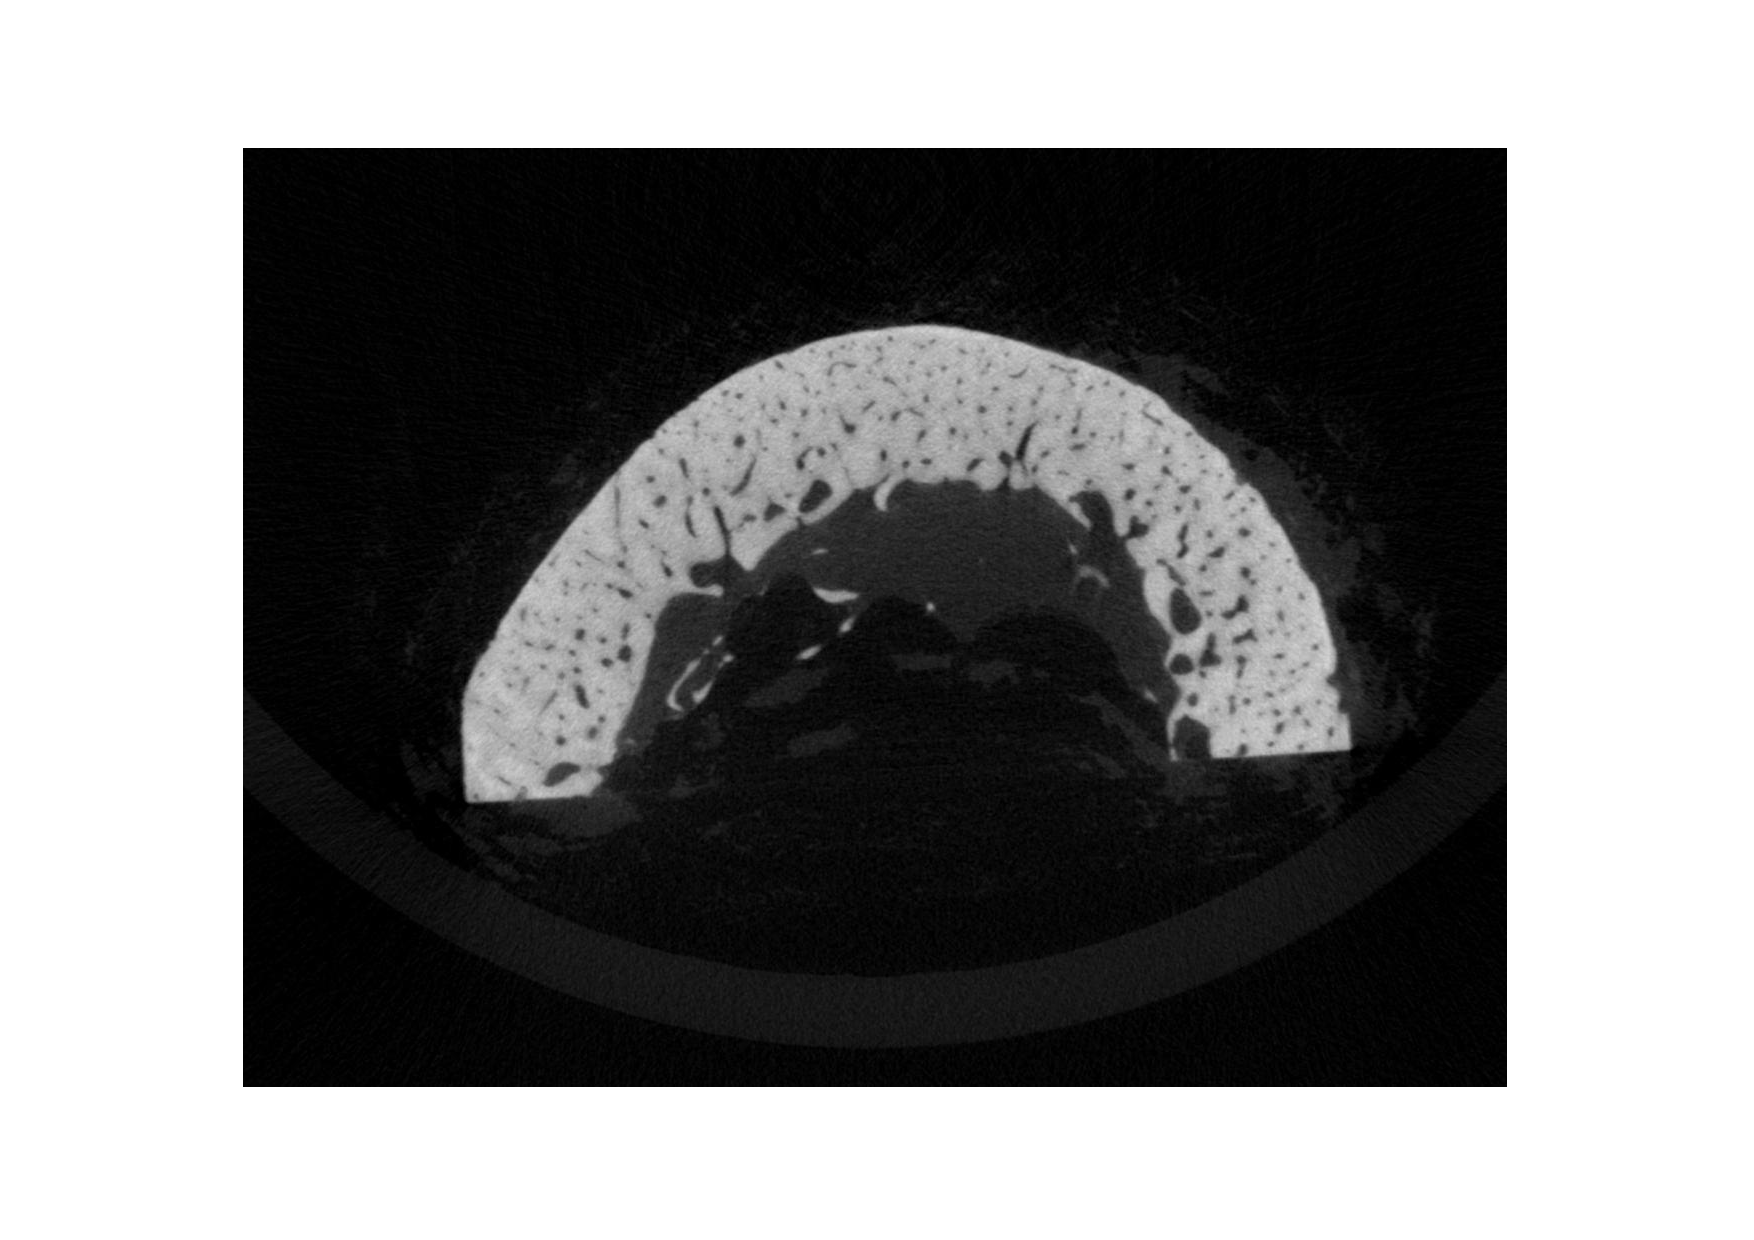
\includegraphics[scale=.5]{images/ImgExt/246-2010_rec0964.pdf}
	\caption{Real sample of $\mu$-CT image obtained, slice 246 of stack. \textit{France, 2010}.}
	\label{muCT-Image}
\end{figure}



The important aspect for the transducer it is the linear element array which contains several emitters and receiver. 

We model the experimental setting of the transductor applied on a patient as a elastodynamic model defined on the cortical bone, where we neglect the effects at the interface defined by the skin. 

In the case of simulations the number of emitters was fixed to 8 initially, but by the traslation invariance of the elastic wave, the simulation only needed the emision using one emitter (or source), while the receptor where modeled by points in the surface containing the displacement vector.

\subsection{Signal Processing}
Each cycle of masurements consists of a sequential excitation of the $N^E > 0$ number of emitters located at boundaries $\Gamma_{e}$ as will be formalized later, which yield $N^E \times N^R$ time series arrays at each time of measurement.
Such a multichannel series denoted by $\{ S(t,e,r) \}_{(t_n,r) \in N^T\times N^R}\}$ at fixed emitter $e \in \{1, \dots, N^E\}$ is then applied a fast \textit{Fourier} transform obtaining $\{ \hat{S}(f,e,k) \}_{(f,k) \in N^F\times N^K}$\footnote{Which we identify following the literature of mechanics and ultrasound analysis as frequency and wavenumber respectively.}

Such Fourier transformed array $\hat{S}(\cdot, e, \cdot)$ for each emitter are then decomposed by singular values method (SVD), in the form:
\begin{equation*}
    P(e) \hat{D} P(e)^T = \hat{S}(e) \quad \text{ for each } e \in \{1, \dots, N^E \}
\end{equation*}

so that by applying the function over the first $N^E_*$ resonant modes given by:
\begin{equation*}
    L(P(e)) := \sum \limits_{e = 1}^{N^E_*} P(e) \overline{P(e)}
\end{equation*}
it defines the so-called \textit{Lamb} waves (or \textit{Lamb} branches) describing the propagation \footnote{Several studies consider the usage of this kind of curves, as ones mainly used to describe the material destruction and mechanical behavior, and moreover in a non-invasive form.} of the material \cite{Rhee2007}.

An important aspect of such \textit{Lamb} curves is the fact that implicitly contain the overall mechanical behavior of the elastodynamical model, so that define a useful tool for validation and comparison of numerical simulation with respect to real data. 


Over such a domain we consider their behaviour of linear elastodynamic type, defined by a displacement $u(\mathbf{x},t)$ with constitutive equation of linear (following \textit{Hookes} law), with forces $\mathbf{F}(t)$ applied at a section of the surface domain. \\

Formally we consider the following:
The domain $\Omega \subset \mathbb{R}^2$ is assumed sufficiently regular, such that $\partial \Omega := \Gamma_N \cup \Gamma_D$ is Lipschitz where the union is disjoint.
We model the material using the displacement $u(\mathbf{x},t) \in H^1(\Omega)$ with behaviour of linear elastic type subjected to surface forces $\mathbf{F}(t) \in L^2 (0, T)$, i.e., the material obeys the following initial boundary value problem:

\begin{align*}
    \rho (\mathbf{x}) \partial_{tt} u(\mathbf{x},t) - \nabla \cdot \sigma (u) & = \mathbf{0}, \text{ in } \Omega \times (0, T) \\
    \sigma(u(\mathbf{x},t))_{ij} &= \mathbf{C}_{ijkl} \mathbf{e}_{kl}(u(\mathbf{x},t)), \text{ in } \Omega \times (0, T) \\
    u(\mathbf{x},t) &= \mathbf{0}, \text{ on } \Gamma_D \times (0, T) \\
    \sigma(u(\mathbf{x},t)) \cdot n &= \mathbf{F}(t), \text{ on } \Gamma_N \times (0,T)
\end{align*}

where $\mathbf{C}(\mathbf{x})$ denotes the elasticity tensor and $\mathbf{e}(u(\mathbf{x},t)) = \frac{1}{2}\big( \nabla u(\mathbf{x},t) + \nabla u(\mathbf{x},t)^{T}$ denotes the symmetric gradient.

\section{Main assumptions and Modelling Multiscale}
Let a bounded domain $\Omega \subset \mathbb{R}^d$ ($d = 2,3$) represent the composed material under study, modelled by an incompressible, elastic matrix and several inclusion defining the so-called mesoscale being modeled mechanically by an elastic of cylindrical shape periodically distributed.
For the sake of the experimental setting under consideration, the exterior boundary $\partial \Omega$ is decomposed as
\begin{equation*}
	\partial \Omega = \Gamma_D \dot\cup \Gamma_N
\end{equation*}
denoting $\Gamma_D, \Gamma_N$ the Dirichlet and Neumann part of the exterior boundary respectively.

Furthermore, let the small parameter $0 < \epsilon \ll 1$ denote the aspect ratio between the macroscopic variable $\mathbf{x} \in \Omega$ and the microscopic one $\mathbf{y}$ in the form: $\mathbf{y} = \frac{\mathbf{x}}{\epsilon}$ being $\mathbf{y} \in \mathbf{Y}$ and $\mathbf{Y} = (0,1)^d$ the cell structure. In this configuration, the unitary cell $\mathbf{Y}$, can be decomposed as
\begin{equation*}
	\mathbf{Y} = \mathbf{Y}_m \cup \Gamma \cup \mathbf{Y}_p 
\end{equation*}
where $\mathbf{Y}_m$ and $\mathbf{Y}_p$ are defined as the domains occupied by the matrix and porous part respectively, and $\Gamma$ denotes the interface between them\footnote{This model is inspired in the development of the Homogenization of the elastic operator in a porous media proposed on \cite{christensen1982theory}. Nevertheless, this kind of configurations are typical in the two-scale homogenization literature \cite{panasenko2005multi-scale}, \cite{Boughammoura2013} to mention updated references.}.

Such a cell is assumed to be periodically distributed along the material, defining its highly oscillatory structure, suitable to use the the Homogenization framework. We consider the composite material of study with elastic properties having oscillation rate $\epsilon$, represented in the domain decomposition:
\begin{equation*}
	\overline{\Omega}^{\epsilon} = (\overline{\Omega}\setminus \Omega_1^{\epsilon}) \cup \overline{\Omega}^{\epsilon}_1
\end{equation*}
where we have defined
\begin{equation*}
    \overline{\Omega}^{\epsilon}_1 = \bigcup_{\mathbf{x} \in \mathbf{T}_{\epsilon}} \epsilon ( \mathbf{x} + \mathbf{Y} )
\end{equation*}
being the tessellation $\mathbf{T}_{\epsilon}$ the subset in $\mathbb{Z}^d$ of all points satisfying the conditions
\begin{equation*}
    \epsilon (\mathbf{x} + \mathbf{Y}) \subset \Omega, \quad \rho(\epsilon(\mathbf{x}+\mathbf{Y}), \partial \Omega) \geq \epsilon
\end{equation*}

Let us note in particular that for fixed $\epsilon >0$ and all $\mathbf{x} \in \Omega$ we have a unique decomposition $\mathbf{x}/\epsilon = \mathbf{x}_{\mathbf{T}_{\epsilon}(\mathbf{x})} + \mathbf{y}$ where $\mathbf{x}_{\mathbf{T}_{\epsilon}(\mathbf{x})}$ denotes the element in $\Omega$ of the tessellation.

The above considerations let us define finally the material coefficients defined as second order rank tensors for component $i,j,k,l \in \{1,\dots, d\}$ in the form:
\begin{equation*}
    C_{ijll}(\frac{\mathbf{x}}{\epsilon}) = C_{ijkl}(\mathbf{y}) \quad \text{for } \frac{\mathbf{x}}{\epsilon} = \mathbf{x}_{\mathbf{T}_{\epsilon}(\mathbf{x})} + \mathbf{y}, \, \mathbf{x} \in \Omega_1^{\epsilon}
\end{equation*}
and being $C_{ijkl}(\frac{\mathbf{x}}{\epsilon}) = 0$ if $\mathbf{x} \in \overline{\Omega} \setminus \Omega_1^{\epsilon}$.
ADD FIGURES OF THE HOMOGENIZATION IDEALIZATION!!

\begin{rem}
We model the material confined within the inclusion as a elastic (emulating a mechanical behavior of blood mixture mainly made of saturated static fluid) with volume $\epsilon^d \vert \mathbf{Y}_p \vert$ embedded in a elastic material (modeled mainly of hydroxipatite and collagen) filling a unit cell of volume $\epsilon^d \vert \mathbf{Y} \vert$.
We define, after scaling, the porosity associated to the material as the fraction of volume occupied by the gas in the unitary cell, i.e., 
\begin{equation*}
\phi = \frac{\vert \mathbf{Y}_p \vert}{\vert \mathbf{Y} \vert} = \vert \mathbf{Y}_p \vert
\end{equation*}
which will define the material coefficients dependent of such parameters.
\end{rem}


